\begin{frame}
\frametitle{$\photon+\text{jet}$ events: Feynman graphs examples}
~\hfill
\begin{fmffile}{gq_qGamma_S}\fmfstraight
\begin{fmfchar*}(20,20)
  \fmfleft{i1,i2}
  \fmfright{o1,o2}
  \fmf{gluon}{i2,v1}
  \fmf{fermion}{i1,v1,v2,o2}
  \fmf{photon}{v2,o1}
  \fmflabel{\gluon}{i2}
  \fmflabel{\quark}{i1}
  \fmflabel{\quark}{o2}
  \fmflabel{\photon}{o1}
  \fmfdot{v1,v2}
\end{fmfchar*}
\end{fmffile}
\hfill\hfill\hfill
\begin{fmffile}{gq_qGamma_T}\fmfstraight
\begin{fmfchar*}(20,20)
  \fmfleft{i1,i2}
  \fmfright{o1,o2}
  \fmf{gluon}{i2,v2}
  \fmf{fermion}{i1,v1,v2,o2}
  \fmf{photon}{v1,o1}
  \fmflabel{\gluon}{i2}
  \fmflabel{\quark}{i1}
  \fmflabel{\quark}{o2}
  \fmflabel{\photon}{o1}
  \fmfdot{v1,v2}
\end{fmfchar*}
\end{fmffile}
\hfill\hfill\hfill
\begin{fmffile}{qq_gGamma}\fmfstraight
\begin{fmfchar*}(20,20)
  \fmfleft{i1,i2}
  \fmfright{o1,o2}
  \fmf{gluon}{v2,o2}
  \fmf{fermion}{i1,v1,v2,i2}
  \fmf{photon}{v1,o1}
  \fmflabel{\antiquark}{i2}
  \fmflabel{\quark}{i1}
  \fmflabel{\gluon}{o2}
  \fmflabel{\photon}{o1}
  \fmfdot{v1,v2}
\end{fmfchar*}
\end{fmffile}
\hfill~

\pause
\vfill

\manip Only 2 \og particles \fg{} (physics objects) in final state:
\begin{itemize}
\item photon (well known);
\item jet (to calibrate).
\end{itemize}
\manip No neutrino $\Rightarrow$ no real \MET.
\end{frame}

\begin{frame}
\frametitle{$\photon+\text{jet}$ events: what it looks like}
\begin{center}
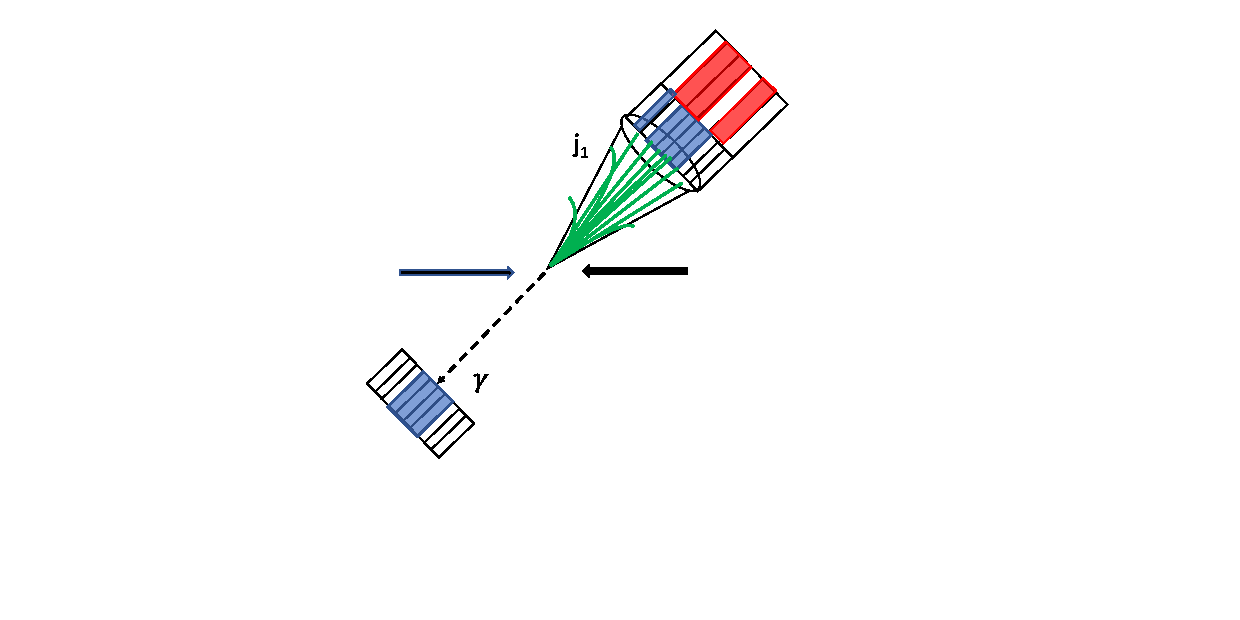
\includegraphics[width=\graphw,height=\graphh,keepaspectratio, trim = 5cm 2.5cm 7.5cm .5cm, clip]{\PhDthesisdir/slides/JERC/JEC_Principe/Gamma_plus_jet_basic_event.pdf}
\end{center}
\end{frame}
